\documentclass[11pt,a4paper]{article}

\usepackage[utf8]{inputenc}
\usepackage[T1]{fontenc}
\usepackage[english]{babel}
\usepackage[a4paper,margin=2.4cm]{geometry}

\usepackage{amsmath, amssymb, amsthm}
\usepackage{mathtools}
\usepackage{booktabs}
\usepackage{tabularx}
\usepackage{array}
\usepackage{caption}
\usepackage{float}
\usepackage{enumitem}
\usepackage{microtype}
\usepackage{xcolor}
\usepackage{listings}
\usepackage{fancyhdr}
\usepackage{titlesec}
\usepackage{tikz}
\usetikzlibrary{positioning, arrows.meta, fit, backgrounds, calc, shapes.geometric}
\usepackage[hidelinks]{hyperref}

%  ---  Palette shared with the companion report  ---
\definecolor{ink}{RGB}{26,30,36}
\definecolor{slate}{RGB}{92,101,112}
\definecolor{mist}{RGB}{233,235,238}
\definecolor{rulegrey}{RGB}{188,194,201}
\definecolor{steel}{RGB}{47,72,102}
\definecolor{steellight}{RGB}{124,146,172}
\definecolor{signal}{RGB}{160,32,45}

\hypersetup{
    colorlinks=true,
    linkcolor=steel,
    citecolor=steel,
    urlcolor=steel,
    pdftitle={Executing Epistemic Policies on ROS 2},
    pdfauthor={Haniel Ulises},
}

\color{ink}

\setlength{\headheight}{22pt}
\pagestyle{fancy}
\fancyhf{}
\fancyhead[L]{\small\textcolor{slate}{\itshape Executing Epistemic Policies on ROS 2}}
\fancyhead[R]{\small\textcolor{slate}{\thepage}}
\renewcommand{\headrulewidth}{0.4pt}
\renewcommand{\headrule}{\hbox to\headwidth{\color{rulegrey}\leaders\hrule height \headrulewidth\hfill}}

\titleformat{\section}{\normalfont\large\bfseries\color{ink}}{\thesection}{0.7em}{}
\titleformat{\subsection}{\normalfont\normalsize\bfseries\color{ink}}{\thesubsection}{0.7em}{}
\titleformat{\paragraph}[runin]{\normalfont\bfseries\color{slate}}{}{0em}{}[.]

\captionsetup{font=small, labelfont={bf,color=slate}, textfont=footnotesize}

\theoremstyle{definition}
\newtheorem{definition}{Definition}

\lstdefinestyle{sys}{
    backgroundcolor=\color{mist},
    basicstyle=\ttfamily\scriptsize\color{ink},
    keywordstyle=\color{steel}\bfseries,
    commentstyle=\color{slate}\itshape,
    stringstyle=\color{slate},
    morecomment=[l]{\#},
    morekeywords={executor,ros__parameters,bt_builder_plugin,bt_node_plugins,
        planner,plan_solver_plugins,EPISTEMIC,conditional_plan,action_mapping,
        Sequence,ReactiveSequence,CheckKnowledge,ApplyEpistemicUpdate,
        EpistemicSwitch,CheckEpistemicGoal,ExecuteAction,true,false,ok,refused},
    frame=single,
    rulecolor=\color{rulegrey},
    framesep=5pt,
    xleftmargin=6pt,
    xrightmargin=0pt,
    breaklines=true,
    showstringspaces=false,
    columns=fullflexible,
    captionpos=b,
}
\lstset{style=sys}

%  ---  Notation  ---
\newcommand{\Ag}{\mathcal{A}}
\newcommand{\Mod}{\mathcal{M}}
\newcommand{\Ev}{\mathcal{E}}
\newcommand{\prd}{\otimes}
\newcommand{\Kop}[1]{K_{#1}}
\newcommand{\Kw}[1]{\mathit{Kw}_{#1}}
\newcommand{\code}[1]{\texttt{\small #1}}

\begin{document}

\begin{titlepage}
\centering
\vspace*{2.4cm}
{\color{rulegrey}\rule{\textwidth}{0.8pt}}\\[0.9cm]
{\LARGE\bfseries Executing Epistemic Policies\\[0.25cm] on ROS 2\par}
\vspace{0.5cm}
{\large\color{slate} A Behaviour-Tree Architecture for DEL Plans,\\ with an Epistemic State Service\par}
\vspace{0.7cm}
{\color{rulegrey}\rule{\textwidth}{0.8pt}}\\[1.4cm]

{\large Haniel Ulises\par}
\vspace{0.3cm}
{\color{slate} Epistemic Robotics}\\
\vspace{0.15cm}
{\color{slate}\today}

\vfill
\begin{minipage}{0.86\textwidth}
\small\color{slate}
\textbf{Abstract.}\ A planner that reasons about knowledge returns a policy, not
a plan: after a sensing action the correct continuation depends on what was
observed, and some preconditions are statements about what an agent knows
rather than about what is true. Neither is expressible in the execution model
of PlanSys2, whose behaviour trees render a plan as a sequence of guarded
actions and whose conditions are checked against a store of facts. This report
describes an execution layer that closes that gap without displacing the
classical one. A policy is carried in additional fields of the existing plan
message, so that planner and executor continue to exchange one type; it is
rendered as a behaviour tree in which the PlanSys2 action subtree survives
unchanged, wrapped in a knowledge guard, a Dynamic Epistemic Logic product
update, and a control node that branches on the observed outcome; and the
conditions those nodes ask about are answered by an epistemic state service
that holds a pointed Kripke model and advances it by executed actions. The
architecture is additive: a plan that never branches renders as the sequence
PlanSys2 would have built, and the executor acquires no dependency on any of
it. We report the design, its failure semantics, and its verification,
including a traced execution in which one agent comes to know the value of a
proposition while another, present but not observing, does not.
\end{minipage}
\vspace{2cm}
\end{titlepage}

\tableofcontents
\newpage

% ─────────────────────────────────────────────────────────────
\section{Introduction}

Planning under partial observability produces objects that classical execution
machinery cannot represent. Two of them matter here.

The first is the shape of the plan. A solution to a planning problem over a
multi-pointed epistemic state is a \emph{policy}: a tree whose branch points are
the designated events of sensing actions and whose leaves satisfy the goal. Any
serialisation of it as a sequence retains one branch and, in doing so, asserts
that the world will take that contingency.

The second is the nature of its conditions. An epistemic plan is built around
formulas such as $\Kw{A}\,\mathit{tails}$ --- \emph{$A$ knows whether the coin
lies tails} --- which is not a proposition about the coin. No valuation of
predicates records it, and so no store of facts can be asked. This is precisely
the distinction that makes an epistemic planner worth having: a robot that must
sense before committing is one whose plan turns on what it will know, not on
what will be true.

PlanSys2~\cite{plansys2} executes a plan by rendering it as a behaviour tree,
one subtree per action, each surrounding its action with the PDDL conditions
that guard it. The model is a good one, and nothing in this report replaces it.
What follows is an account of what has to be added around it, and of where the
dependency between the two is allowed to fall.

\paragraph{Contributions} This report describes: (i) an additive extension of
the plan message that carries a policy without forking either interface between
planner and executor (\S\ref{sec:wire}); (ii) a behaviour-tree architecture in
which the classical action subtree is preserved and surrounded by three
epistemic nodes, with failure semantics that prefer replanning to guessing
(\S\ref{sec:tree}); (iii) an epistemic state service that is to knowledge what
the problem expert is to facts (\S\ref{sec:state}); and (iv) a package structure
in which only one small component depends on the executor
(\S\ref{sec:structure}), together with its verification (\S\ref{sec:verif}).

% ─────────────────────────────────────────────────────────────
\section{Background}

\subsection{Epistemic states and policies}

An epistemic state is a multi-pointed Kripke model
$\Mod = (W, \{R_i\}_{i\in\Ag}, V, W^{*})$: the worlds the agents consider
possible, one accessibility relation per agent, a valuation, and the designated
set $W^{*}$ of candidates for the actual world. An action is an event model
$\Ev = (E, \{Q_i\}, \mathrm{pre}, \mathrm{post}, E^{*})$ applied by product
update~\cite{bms}:
\[
  \Mod \prd \Ev \;=\;
  \bigl(\{(w,e) : \Mod,w \models \mathrm{pre}(e)\},\;
  (w,e)R'_i(v,f) \iff wR_iv \wedge eQ_if,\;
  V',\; W^{*}\!\times\!E^{*}\bigr).
\]
An action with a single designated event is \emph{ontic}: its effect on the
model is determined by the action alone. An action with several is
\emph{sensing}: the product splits into one successor state per designated
event, and which of them obtains is a fact about the world rather than about the
model. A solution is therefore a policy, and this asymmetry --- ontic actions
continue, sensing actions branch --- is what the execution layer must honour.

\subsection{The PlanSys2 execution model}

PlanSys2 renders each plan item as a subtree that waits for the action's at-start
requirements, applies its at-start effects, executes the action while its
over-all requirements hold, then checks and applies its at-end effects. Actions
are identified by a key formed from the action expression and its start time in
milliseconds, and it is by this key that a tree node finds the action executor it
drives. Both facts matter later: the subtree is what we preserve, and the key is
what a policy can inadvertently collide (\S\ref{sec:keys}).

% ─────────────────────────────────────────────────────────────
\section{A policy on the wire}
\label{sec:wire}

Two interfaces separate the planner from the executor, and both are typed on the
flat plan message: the solver plugin returns one, and the tree builder consumes
one. Forking either would fork the system. Instead the policy travels in
additional fields of the message itself (Table~\ref{tab:fields}).

\begin{table}[H]
\centering
\small
\begin{tabularx}{\textwidth}{@{}lX@{}}
\toprule
\textbf{Field} & \textbf{Content} \\
\midrule
\code{children}               & one continuation per possible outcome, by item index \\
\code{outcomes}               & the observation selecting each, in the same order \\
\code{sensing}                & whether the outcome must be observed at all \\
\code{knowledge\_requirements}& the epistemic conditions the action requires \\
\code{epistemic\_action}      & the action's name in the planner's own vocabulary \\
\bottomrule
\end{tabularx}
\caption{Fields added to the plan item. A classical planner sets none of them.}
\label{tab:fields}
\end{table}

\paragraph{Two vocabularies} The last field deserves comment. A grounder emits an
action as a single token, \code{pickup-A-hold\_r2}, whereas the executor parses
\code{(pickup r2 A)} into a name and parameters and resolves the name against the
PDDL domain to find the behaviour tree that drives the hardware. These are two
vocabularies, not two spellings of one, and no convention recovers the parameter
order that the grounded name does not record. Translation is therefore performed
through an explicit map, and an action the map does not cover fails the planning
request rather than reaching the executor as a name it cannot resolve. Both names
survive on the item: the translated one for the executor, the grounded one for
the epistemic state, which needs it to find the action's event model.

\paragraph{The sequential reading} When no item names a continuation, the plan is
read as PlanSys2 writes it: item $i$ followed by item $i+1$. This reading is
plan-wide rather than per item, because an item with no continuation is also how
a policy says \emph{this branch ends here}, and the two cannot be distinguished
one item at a time. A planner that links any node must therefore link all of
them. The consequence is that every plan is a policy, and the distinction that
matters is not classical versus epistemic but whether the policy branches.

\subsection{Unique execution keys}
\label{sec:keys}

Since the executor keys its table of running actions by expression and start
time, two policy nodes bearing the same action at the same time collide onto one
entry, and one action executor is then driven from two places. The fault is
invisible under test: branches are alternatives, so the collision has no effect
until the day execution takes the second one. Start times are therefore assigned
so that no two nodes share a key, each node beginning strictly after its parent
ends; the property is asserted directly against a reproduction of the executor's
own key construction.

% ─────────────────────────────────────────────────────────────
\section{The behaviour tree}
\label{sec:tree}

Each policy node renders as the PlanSys2 action subtree --- unchanged, driving
the same action performers against the same problem expert --- surrounded by
three constructs that a sequence cannot express (Figure~\ref{fig:tree}).

\begin{figure}[H]
\centering
\begin{tikzpicture}[
  font=\small,
  box/.style={draw=rulegrey, fill=white, rounded corners=1pt,
              minimum height=8mm, text width=104mm, align=left, inner sep=2.4mm},
  ebox/.style={box, draw=signal, line width=0.7pt},
  pbox/.style={box, fill=mist},
  bbox/.style={draw=rulegrey, fill=white, rounded corners=1pt,
               text width=48mm, align=left, inner sep=2.2mm, minimum height=11mm},
  arr/.style={-{Stealth[length=1.6mm]}, draw=slate}
]

\node[ebox] (guard) {\textbf{CheckKnowledge}\\[1pt]
  {\scriptsize\color{slate}\texttt{(K A looking\_A)} --- asked of the epistemic state}};

\node[pbox, below=3mm of guard] (ps) {\textbf{\color{slate}PlanSys2, unchanged}\\[1pt]
  {\scriptsize\ttfamily WaitAtStartReq $\rightarrow$ ApplyAtStartEffect}\\
  {\scriptsize\ttfamily ReactiveSequence[\,CheckOverAllReq, ExecuteAction\,]}\\
  {\scriptsize\ttfamily CheckAtEndReq $\rightarrow$ ApplyAtEndEffect}};

\node[ebox, below=3mm of ps] (upd) {\textbf{ApplyEpistemicUpdate}\\[1pt]
  {\scriptsize\color{slate}$\Mod \prd \Ev$; reports the observed outcome}};

\node[ebox, below=3mm of upd] (sw) {\textbf{EpistemicSwitch}\\[1pt]
  {\scriptsize\color{slate}\texttt{outcomes = e-peek-pos ; e-peek-neg}}};

\node[bbox, anchor=north east] (b1) at ([shift={(-2mm,-9mm)}]sw.south)
  {{\scriptsize\color{signal}\texttt{observed e-peek-pos}}\\[2pt]
   {\scriptsize Sequence, node 1\\ \texttt{(shout-tails A)}}};
\node[bbox, anchor=north west] (b2) at ([shift={(2mm,-9mm)}]sw.south)
  {{\scriptsize\color{signal}\texttt{observed e-peek-neg}}\\[2pt]
   {\scriptsize AlwaysSuccess ---\\ the policy ends here}};

\draw[arr] (guard) -- (ps);
\draw[arr] (ps) -- (upd);
\draw[arr] (upd) -- (sw);
\draw[arr] (sw.south) -- ++(0,-4mm) -| (b1.north);
\draw[arr] (sw.south) -- ++(0,-4mm) -| (b2.north);

\begin{scope}[on background layer]
  \node[draw=ink, line width=0.8pt, fit=(guard)(ps)(upd)(sw)(b1)(b2),
        inner sep=3.4mm, rounded corners=1pt] (outer) {};
\end{scope}

\node[ebox, below=6mm of outer] (goal) {\textbf{CheckEpistemicGoal}\\[1pt]
  {\scriptsize\color{slate}$\Kw{A}\,\mathit{tails}$ --- asked once, of the state that resulted}};

\draw[arr] (outer.south) -- (goal.north);

\end{tikzpicture}
\caption{One policy node rendered as a behaviour tree. The grey block is the
PlanSys2 action subtree, preserved verbatim; the outlined nodes are the
epistemic additions. A node with a single continuation renders without a switch,
so a plan that never branches yields the flat sequence PlanSys2 would build.}
\label{fig:tree}
\end{figure}

\subsection{The three additions}

\paragraph{CheckKnowledge} The counterpart of \code{CheckOverAllReq} for
conditions the problem expert cannot answer. It is a distinct node because it
consults a distinct store: facts and knowledge are different kinds of thing, and
collapsing them would either invent predicates for knowledge or silently accept
conditions nothing has checked. A requirement that cannot be evaluated fails the
node, and is reported differently from one that is evaluated and does not hold:
the first says we cannot tell, the second says the plan is wrong.

\paragraph{ApplyEpistemicUpdate} The counterpart of \code{ApplyAtEndEffect}, one
level up. An action changes what agents know by more than its own effects: a
public announcement informs every observer, and an observation that finds nothing
still eliminates worlds. Performing the update as a tree node --- rather than
folding it into effect application --- keeps the guard on the next action checked
against the state this action produced. The update is applied once per execution
of its node, since product update is not idempotent: applying an announcement
twice asserts that the agents were told twice.

\paragraph{EpistemicSwitch} A control node with no classical counterpart. It
reads the outcome the update reported and ticks the continuation planned for it,
matching outcomes to children by position. Three properties are deliberate. A
branch already running is not re-selected, since halting a running action to
restart it would interrupt the robot mid-action. A tree whose outcome list and
child count disagree fails rather than indexing past its children. And an outcome
the policy does not list fails the node:

\begin{quote}\itshape\color{slate}
Every branch was constructed for a different belief; running one for an
observation it was not built for is a robot acting confidently on a belief
nothing supports.
\end{quote}

\noindent The failure propagates to the executor, whose response to a failed plan
is to replan --- from the state that actually resulted, which is the correct
response to a world that did something the plan did not anticipate.

\subsection{Goal checking}

The goal is checked once, after the policy, rather than at each leaf. Every leaf
was believed to satisfy the goal, but that belief was formed against the model at
planning time; if execution diverged, a policy can run to completion in a branch
that no longer establishes anything. The goal formula travels on the plan
message, because an epistemic goal is not the PDDL goal the executor already
holds. A tree carrying no epistemic goal --- a classical plan --- passes this
node unconditionally.

% ─────────────────────────────────────────────────────────────
\section{The epistemic state}
\label{sec:state}

The tree requires something to ask. A lifecycle node holds a pointed Kripke model
and exposes three services, which are exactly the three questions that executing
a policy raises (Table~\ref{tab:services}).

\begin{table}[H]
\centering
\small
\begin{tabularx}{\textwidth}{@{}lX@{}}
\toprule
\textbf{Service} & \textbf{Question} \\
\midrule
\code{load\_task}     & be the model of \emph{this} grounded task \\
\code{check\_formula} & does this epistemic formula hold now? \\
\code{apply\_action}  & this action has run: update, and report what was observed \\
\bottomrule
\end{tabularx}
\caption{The epistemic state service. Its relation to knowledge is that of the
problem expert to facts.}
\label{tab:services}
\end{table}

The model advances by executed actions rather than by observation of the world,
which is what makes it a belief state rather than a log. Disagreement with
reality therefore surfaces at \code{apply\_action}, as an action that is not
applicable or an outcome the model cannot produce --- reported as an error rather
than absorbed by overwriting the model.

\subsection{Formulas across a process boundary}

Formulas are hash-consed within a planning process, so structural identity is
pointer identity and comparison is constant time. Those identifiers are
process-local and cannot cross a service boundary. Conditions therefore travel as
text over the task's vocabulary --- \code{(K r1 (clear corridor))},
\code{(Kw A tails)} --- written by the planner and parsed by the state.

Nothing but the agreement of those two procedures connects them, so the agreement
is tested directly: every goal and every action precondition of each benchmark
task is rendered and parsed back, and the result compared as a \emph{formula}
rather than as a string. A name absent from the task is rejected rather than
interned as a fresh symbol, since it indicates that policy and state disagree
about which problem is being solved.

\subsection{Who determines the outcome}

For an ontic action the update is determined and the response reports no outcome.
For a sensing action the state splits into one successor per designated event,
and the question of which obtains is about the world. Three cases arise:

\begin{enumerate}[leftmargin=*, itemsep=2pt]
  \item An observation is supplied and names a possible outcome: it is applied.
  \item No observation is supplied and the state designates a single world: the
        outcome is determined, and the response reports it.
  \item No observation is supplied and several worlds are designated: the model
        genuinely does not know. The request fails.
\end{enumerate}

\noindent The third case is a design commitment rather than a limitation.
Selecting a branch on a model's convenience, when the model has not the
information to select one, is exactly the error the architecture exists to
prevent.

% ─────────────────────────────────────────────────────────────
\section{Structure}
\label{sec:structure}

Extending an executor ordinarily entails depending on it. That was worth
avoiding: a package requiring \code{plansys2\_executor} can be built only against
the fork that provides it, whereas a package that does not can be built and
tested against a released distribution.

\begin{table}[H]
\centering
\small
\begin{tabularx}{\textwidth}{@{}lXc@{}}
\toprule
\textbf{Package} & \textbf{Contents} & \textbf{Needs executor} \\
\midrule
\code{plansys2\_epistemic\_msgs}       & the three service definitions & no \\
\code{plansys2\_epistemic\_executor}   & policy, tree rendering, four nodes, the state & no \\
\code{plansys2\_epistemic\_bt\_builder}& the tree-builder plugin & yes \\
\bottomrule
\end{tabularx}
\caption{Only the builder requires the executor's plugin interface.}
\label{tab:packages}
\end{table}

The nodes reach the executor through a generic hook rather than a special case: a
parameter naming behaviour-tree node libraries to be loaded before a tree is
built, together with the plan already published on the tree's blackboard. The
executor consequently links against none of the epistemic code and contains
nothing that knows what an epistemic node is; it loads a library and finds four
more node types available.

\begin{lstlisting}[caption={The entire configuration, above the ordinary PlanSys2 parameters.}]
executor:
  ros__parameters:
    bt_builder_plugin: "EpistemicBTBuilder"
    bt_node_plugins:   ["libplansys2_epistemic_bt_nodes.so"]
\end{lstlisting}

% ─────────────────────────────────────────────────────────────
\section{Verification}
\label{sec:verif}

\begin{table}[H]
\centering
\small
\begin{tabular}{@{}lrr@{}}
\toprule
\textbf{Package} & \textbf{Tests} & \textbf{Failures} \\
\midrule
\code{plansys2\_epistemic\_planner}  & 38 & 0 \\
\code{plansys2\_epistemic\_executor} & 39 & 0 \\
\code{plansys2\_epistemic\_msgs}     &  5 & 0 \\
\midrule
Total, from a clean build of six packages & 82 & 0 \\
\bottomrule
\end{tabular}
\caption{Automated verification.}
\label{tab:tests}
\end{table}

Three of these checks carry more weight than their number suggests. Every
rendered tree is submitted to the behaviour-tree library's own parser, since a
tree that fails to parse is worthless however well formed it appears. The
formula round trip is compared as described in \S\ref{sec:state}. And the node
library is loaded exactly as the executor loads it, so that the extension
mechanism is tested rather than assumed.

\subsection{A traced execution}

The following is a verbatim trace against the running state node, on a
multi-pointed variant of the coin-in-the-box domain in which both coin worlds are
designated and the goal is $\Kw{A}\,\mathit{tails}$.

\begin{lstlisting}[caption={Service responses, in order.}]
# A must come to know whether the coin lies tails. It starts not knowing.
check_formula  (Kw A tails)        -> holds=false

# The box is shut, so looking is not yet possible. The guard says so.
apply_action   peek_A              -> refused: not applicable in the current
                                      epistemic state
apply_action   open_A              -> ok; 4 worlds, 2 designated

# A may now look. But two worlds are designated, so the model cannot know
# which outcome the world produced, and declines to choose one.
apply_action   peek_A              -> refused: 2 possible outcomes here and
                                      none was observed

# The robot reports what it saw. The model narrows to a single world.
apply_action   peek_A  e-peek-pos  -> ok; outcome=e-peek-pos
                                      6 worlds, 1 designated

check_formula  (Kw A tails)        -> holds=true    # A looked
check_formula  (Kw B tails)        -> holds=false   # B was not looking
\end{lstlisting}

The final pair is the substantive result. $A$ observed and now knows; $B$ was
present and does not. Quasi-private sensing survives intact from the event model,
through the product update, to a service answer that a behaviour tree node can
act upon. The two refusals are equally the design operating as intended: a guard
that will not admit an inapplicable action, and a model that will not fabricate
an observation it cannot have.

\subsection{What is not covered}

Two things are exercised only in continuous integration, where a full system is
available: the four nodes ticking against a live state under a complete stack,
and the builder operating inside a running executor. The trace above was produced
against the real state node, driven manually.

% ─────────────────────────────────────────────────────────────
\section{Limitations and further work}

\paragraph{Observation binding} The outcome of a sensing action is supplied on a
port that a domain-specific tree binds to whatever its performer reports. Until
that port is bound to real perception, the branch a robot takes is chosen by a
model that happens to designate a single world rather than by its sensors.
Binding it is the step that converts this architecture into a demonstration, and
it is the immediate next piece of work.

\paragraph{Concurrency} The policy is executed as a tree of sequential nodes.
PlanSys2's temporal builders exploit the partial order between actions to run
independent ones concurrently; a policy fixes the order along each branch, so
there is at present nothing for such a graph to decide. Recovering concurrency
\emph{within} a branch is possible in principle and untouched here.

\paragraph{Replanning} A failed switch surfaces to the executor as a failed plan,
which is the correct signal, but the loop that replans from the resulting
epistemic state --- rather than from the initial one --- has not been closed. The
state service already exposes what such a loop requires.

% ─────────────────────────────────────────────────────────────
\begin{thebibliography}{9}
\small

\bibitem{plansys2}
F.~Mart\'in, J.~Gin\'es, F.~J.~Rodr\'iguez-Lera, and V.~Matell\'an.
\newblock PlanSys2: A Planning System Framework for ROS2.
\newblock \emph{IEEE/RSJ International Conference on Intelligent Robots and
Systems (IROS)}, 2021.

\bibitem{bms}
A.~Baltag, L.~S.~Moss, and S.~Solecki.
\newblock The Logic of Public Announcements, Common Knowledge, and Private
Suspicions.
\newblock \emph{Proceedings of TARK}, 1998.

\bibitem{bolander}
T.~Bolander and M.~B.~Andersen.
\newblock Epistemic Planning for Single- and Multi-Agent Systems.
\newblock \emph{Journal of Applied Non-Classical Logics}, 21(1):9--34, 2011.

\bibitem{btcpp}
M.~Colledanchise and P.~\"Ogren.
\newblock \emph{Behavior Trees in Robotics and AI: An Introduction}.
\newblock CRC Press, 2018.

\end{thebibliography}

\end{document}
